% Provenance (never printed): see sources/outline_sources.md (Year 3:
% energy-balance models, the one-layer model recalled; ice-albedo feedback
% and multiple equilibria; how general circulation models are built and
% evaluated).
% Brief: sources/book5/BRIEFS.md, ch. 22. Curves from
% figdata/bachelor-3/budyko_sellers.py (the zero-dimensional model and
% Budyko's latitudinal model; the brief's ebm_0d is folded into it) and
% two_layer.py. Exercise and problem values in the Book 5 scratch calculator
% calc/ch22.py. The model planet, model X and the ensemble of exercise 12 are
% invented.
\chapter{Model Iklim}\label{ch:b3:climate-models}

Ambil sinar Matahari yang sampai ke Bumi, \qty{340}{W/m^2} yang dirata-ratakan
ke seluruh Bumi, dan hukum untuk inframerah yang dikirim kembali ke antariksa, yang dicocokkan dengan
tiga puluh tahun reanalisis dari observasi. Biarkan albedo planet naik dari albedo
tanah terbuka dan laut ke albedo es seiring permukaan mendingin. Seimbangkan kedua
fluks itu, dan persamaannya memiliki tiga solusi: planet pada
\qty{14}{\celsius}, mendekati rata-rata Bumi yang sebenarnya; planet pada
\qty{8}{\celsius}; dan planet pada \qty{-46}{\celsius}, membeku dari
kutub ke kutub. Model iklim, dari beberapa baris ini sampai program yang
dijalankan pada komputer terbesar, adalah alat untuk menanyakan iklim apa yang dimiliki suatu planet, bagaimana planet itu mencapainya,
dan bagaimana iklim berubah ketika neraca energinya terganggu.
% ledger: nasa:solar-mean, data:b5-ncep-air, data:b3-ncep, budyko69:albedo

\begin{recall}
Benda hitam, hukum Stefan--Boltzmann, efek rumah kaca, dan
model satu lapisan atmosfer ada di buku fisika; albedo dan
anggaran energi Bumi di buku sekolah. Radiasi gelombang panjang keluar,
suhu emisi, dan transpor panas meridional dibahas dalam
volume Tahun 1, di bab tentang radiasi dan transpor panas. Umpan balik es--albedo dan
Bumi bola salju ada di volume Tahun 2, di
bab tentang Bumi Prakambrium; gaya radiatif efektif, parameter
umpan balik iklim $\lambda < 0$, sensitivitas iklim kesetimbangan
(ECS) dan respons iklim transien (TCR) di bab
tentang perubahan iklim antropogenik; prediksi cuaca numerik dan
ansambel prakiraan di bab tentang sistem cuaca. Persamaan
gerak pada Bumi yang berotasi, dengan \omterm{def:b3:gfd-foundations:hydrostatic}{pendekatan hidrostatik}, dibahas dalam
Bab~\ref{ch:b3:gfd-foundations}.
\end{recall}

\section{Neraca energi planet}\label{sec:b3:climate-models:zero-d}

Dirata-ratakan ke seluruh bola dan selama setahun, setiap meter persegi di puncak
atmosfer menerima $Q = S_0/4 = \qty{340}{W/m^2}$, seperempat dari
iradiansi Matahari $S_0 = \qty{1360}{W/m^2}$. Sebagian $\alpha$, yakni
albedo planet, dipantulkan; sisanya, $Q(1 - \alpha)$, diserap dan
harus dikembalikan ke antariksa sebagai inframerah. Benda hitam akan memancarkan $\sigma
T^4$; radiasi gelombang panjang keluar Bumi (OLR) lebih kecil karena
efek rumah kaca, dan pada rentang suhu permukaan yang dijumpai di
Bumi, ia mendekati sebuah garis lurus,
\[
\text{OLR} = A + BT ,
\]
dengan $T$ suhu permukaan dalam derajat Celsius. Pada 1969 Budyko mencocokkan
hukum serupa ke radiasi keluar yang dihitung untuk 260 stasiun, dengan koreksi terhadap
tutupan awan $n$: $I = a + bT - (a_1 + b_1T)n$, $a = 14.0$, $b = 0.14$, $a_1 =
3.0$ dan $b_1 = 0.10$ dalam \unit{kcal.cm^{-2}} per bulan, dengan sebaran di bawah
\qty{5}{\percent}. Dengan tutupan awan rata-rata 0.5, ia memberikan $A =
\qty{199}{W/m^2}$ dan $B = \qty{1.43}{W.m^{-2}.\celsius^{-1}}$. \omterm{def:b3:atmospheric-dynamics:eddy}{Rata-rata zonal}
tahunan NCEP--NCAR Reanalysis~1 untuk 1991--2020, ditimbang menurut luas,
memberikan $A = \qty{211.9}{W/m^2}$ dan $B = \qty{1.816}{W.m^{-2}.\celsius^{-1}}$,
dengan sebaran \qty{10}{W/m^2} di sekitar garis. Nilai-nilai ini dipakai
di bawah ini.
% ledger: nasa:solar-mean, budyko69:olr, data:b5-ncep-air, data:b3-ncep

\begin{definition}[Model keseimbangan energi]\label{def:b3:climate-models:ebm}
Yang disebut \emph{model keseimbangan energi}\index{model keseimbangan energi} adalah model iklim
yang menghitung suhu permukaan --- satu rata-rata global, atau
rata-rata pada setiap lintang --- dari keseimbangan sinar Matahari yang diserap, radiasi
inframerah yang dipancarkan ke antariksa dan, jika suhu bergantung pada lintang, panas
yang dibawa menuju kutub. Dalam bentuk nol-dimensi,
\[
C\,\frac{\mathrm dT}{\mathrm dt} = Q\big(1 - \alpha(T)\big) - (A + BT) ,
\]
dengan $C$ kapasitas kalor per satuan luas bagian sistem yang
menghangat bersama permukaan.
\end{definition}

Dengan $\alpha = 0.30$, kesetimbangan berada pada $T = (238 - 211.9)/1.816 =
\qty{14.4}{\celsius}$; rata-rata luas reanalisis adalah
\qty{14.2}{\celsius}. Gaya $F$, misalnya akibat perubahan karbon
dioksida, menambah ruas kanan. Di dekat kesetimbangan, respons
diatur oleh parameter umpan balik iklim $\lambda$ dari volume Tahun 2:
dengan albedo tetap, $\lambda = -B$.
% ledger: earth:albedo, data:b5-ncep-air

\begin{theorem}[Waktu respons iklim satu kotak]\label{thm:b3:climate-models:response}
Misalkan suatu iklim berada dalam kesetimbangan, dan misalkan gaya konstan $F$ dinyalakan
pada $t = 0$. Jika simpangan $T'$ dari kesetimbangan memenuhi $C\,\mathrm
dT'/\mathrm dt = F + \lambda T'$ dengan $C > 0$ dan $\lambda < 0$ konstan,
maka
\[
T'(t) = -\frac{F}{\lambda}\Big(1 - \mathrm e^{-t/\tau}\Big), \qquad
\tau = -\frac{C}{\lambda} .
\]
Kesetimbangan baru adalah $-F/\lambda$, dan iklim menempuh pecahan $1
- \mathrm e^{-1} = \num{0.63}$ dari perubahan itu dalam waktu $\tau$.
\end{theorem}

\begin{proof}
$T'_\infty = -F/\lambda$ membuat ruas kanan menjadi nol. Selisih
$u = T' - T'_\infty$ memenuhi $C\,\mathrm du/\mathrm dt = \lambda u$, sehingga $u =
u(0)\,\mathrm e^{\lambda t/C}$, dengan $u(0) = F/\lambda$.
\end{proof}

Kapasitas kalor yang penting dalam beberapa tahun adalah kapasitas lapisan atas samudra.
Emulator dua lapisan dari laporan penilaian keenam
Panel Antarpemerintah tentang Perubahan Iklim, dikalibrasi pada 44 model iklim,
memberikan lapisan permukaan $C = \qty{8.1}{W.yr.m^{-2}.\celsius^{-1}}$, yaitu kapasitas
kalor lapisan air laut dengan kedalaman \qty{62}{m}. Dengan $\lambda = -B$, waktu
respons adalah $8.1/1.816 = \num{4.5}\text{ tahun}$. Iklim nyata juga menghangatkan
samudra dalam, jauh lebih lambat; Bagian~\ref{sec:b3:climate-models:two-layer}
menambahkannya.
% ledger: ar6sm7:two-layer, teos10:cp0, data:b5-ncep-air

\section{Es, albedo dan kesetimbangan ganda}\label{sec:b3:climate-models:multiple}

Umpan balik es--albedo dari volume Tahun~2 membuat albedo bergantung pada
suhu. Ambil $\alpha = 0.62$ untuk planet yang permukaannya berada di bawah
$T_I = \qty{-10}{\celsius}$, albedo es dalam model Budyko, $\alpha
= 0.30$ di atas $T_F = \qty{+10}{\celsius}$, serta garis lurus di antaranya,
seiring es surut. Tanjakan ini pilihan bab ini; albedo apa pun yang
meningkat saat planet mendingin memberikan gambaran yang sama.
% ledger: budyko69:albedo, earth:albedo

\begin{definition}[Kesetimbangan iklim ganda; bifurkasi pelana-simpul]\label{def:b3:climate-models:multiple-equilibria}
Model iklim memiliki \emph{kesetimbangan iklim ganda}\index{kesetimbangan iklim ganda}
ketika, untuk kondisi eksternal yang sama, ia memiliki lebih dari
satu keadaan tunak. Suatu kesetimbangan stabil jika simpangan kecil darinya
meluruh, dan tak stabil jika membesar. Yang disebut \emph{bifurkasi
pelana-simpul}\index{bifurkasi pelana-simpul} adalah nilai parameter tempat
satu kesetimbangan stabil dan satu tak stabil bertemu lalu lenyap bersamaan.
\end{definition}

\begin{proposition}[Tiga kesetimbangan dan kestabilannya]\label{prop:b3:climate-models:three}
Tulis $N(T) = Q(1 - \alpha(T)) - (A + BT)$ untuk fluks turun neto. Suatu
kesetimbangan $T^*$, $N(T^*) = 0$, stabil jika $N'(T^*) < 0$ dan tak stabil jika
$N'(T^*) > 0$. Dengan tanjakan di atas, $N' = -B$ pada cabang bola salju dan
cabang bebas es, yang stabil di mana pun ia ada, dan $N' = -B -
Q\,\mathrm d\alpha/\mathrm dT$ pada tanjakan, yang tak stabil bila $Q\,
|\mathrm d\alpha/\mathrm dT| > B$. Untuk $Q = \qty{340}{W/m^2}$ model memiliki
tiga kesetimbangan, \qty{-45.5}{\celsius} (stabil), \qty{7.8}{\celsius}
(tak stabil) dan \qty{14.4}{\celsius} (stabil).
\end{proposition}

\begin{proof}
Di dekat $T^*$, $C\,\mathrm dT'/\mathrm dt = N'(T^*)T'$, yang meluruh jika
$N'(T^*) < 0$ dan membesar jika $N'(T^*) > 0$. Pada tanjakan $\mathrm d\alpha/
\mathrm dT = -0.32/20 = \qty{-0.016}{\celsius^{-1}}$, sehingga $N' = -1.816 + 340
\times 0.016 = \qty{+3.62}{W.m^{-2}.\celsius^{-1}}$. Cabang bola salju,
$T = (340\times0.38 - 211.9)/1.816 = \qty{-45.5}{\celsius}$, berada di bawah
$T_I$; cabang hangat, \qty{14.4}{\celsius}, di atas $T_F$; pada tanjakan,
$340(0.54 + 0.016\,T) = 211.9 + 1.816\,T$ memberikan $T = \qty{7.8}{\celsius}$.
\end{proof}

\begin{omfigure}
\begin{tikzpicture}
\begin{groupplot}[group style={group size=2 by 1, horizontal sep=1.5cm},
  width=0.48\linewidth, height=0.4\linewidth,
  tick label style={font=\scriptsize}, label style={font=\small}, title style={font=\small}]
\nextgroupplot[xlabel={$T$ (\unit{\celsius})}, ylabel={fluks (\unit{W/m^2})},
  xmin=-60, xmax=40, ymin=80, ymax=270, title={keseimbangan pada $Q = \qty{340}{W/m^2}$},
  legend style={font=\scriptsize, at={(0.03,0.97)}, anchor=north west}]
% computed in figdata/bachelor-3/budyko_sellers.py
\addplot[omThm, thick] table[x=T, y=asr] {figdata/out/bachelor-3-budyko_sellers-asr.dat};
\addlegendentry{sinar Matahari terserap}
\addplot[omDef, thick] table[x=T, y=olr] {figdata/out/bachelor-3-budyko_sellers-olr.dat};
\addlegendentry{$A + BT$}
\addplot[only marks, mark=*, mark size=2pt, forget plot] coordinates {(-45.55,129.2) (14.38,238.0)};
\addplot[only marks, mark=o, mark size=2pt, thick, forget plot] coordinates {(7.81,226.07)};
\node[font=\scriptsize, anchor=north west] at (axis cs:-45.55,125) {bola salju};
\draw[black!60] (axis cs:7.81,226.07) -- (axis cs:16,200);
\node[font=\scriptsize, anchor=north west, inner sep=1pt] at (axis cs:16,200) {tak stabil};
\nextgroupplot[xlabel={$S_0$ (\unit{W/m^2})}, ylabel={$T$ (\unit{\celsius})},
  xmin=1000, xmax=2200, ymin=-70, ymax=100, title={kesetimbangan dan histeresis},
  scaled x ticks=false, xticklabel style={/pgf/number format/1000 sep={}}]
\addplot[black!40, densely dotted, forget plot] coordinates {(1360,-70) (1360,100)};
\addplot[omMeth, thick] table[x=S, y=T] {figdata/out/bachelor-3-budyko_sellers-eqwarm.dat};
\addplot[omThm, thick] table[x=S, y=T] {figdata/out/bachelor-3-budyko_sellers-eqcold.dat};
\addplot[black!60, thick, dashed] table[x=S, y=T] {figdata/out/bachelor-3-budyko_sellers-eqmid.dat};
\draw[->, thick, black!70] (axis cs:1314.6,8) -- (axis cs:1314.6,-45);
\draw[->, thick, black!70] (axis cs:2039.4,-8) -- (axis cs:2039.4,77);
\node[font=\scriptsize, anchor=south, black!60, fill=white, inner sep=1pt] at (axis cs:1360,84) {hari ini};
\node[font=\scriptsize, omMeth, anchor=north west] at (axis cs:1700,32) {hangat};
\node[font=\scriptsize, omThm, anchor=north] at (axis cs:1620,-40) {bola salju};
\end{groupplot}
\end{tikzpicture}

\par\smallskip{\small \omterm{def:b3:climate-models:ebm}{Model keseimbangan energi} nol-dimensi dengan
tanjakan es--albedo dan hukum OLR yang dicocokkan dengan NCEP--NCAR Reanalysis~1.
Kiri, sinar Matahari terserap dan inframerah yang dipancarkan untuk sinar Matahari hari ini:
keduanya berpotongan tiga kali; lingkaran terisi stabil, lingkaran terbuka tak stabil.
Kanan, suhu kesetimbangan terhadap konstanta surya, cabang stabil
berupa garis penuh, cabang tak stabil putus-putus. Menurunkan Matahari dari
nilai hari ini mendinginkan planet hangat hingga cabang hangat berakhir pada
\qty{1315}{W/m^2}, dan iklim jatuh ke bola salju; ia tetap beku
hingga Matahari dinaikkan ke \qty{2039}{W/m^2}, saat ia melompat kembali ke
planet yang sangat panas, jauh di luar rentang tempat OLR garis lurus
berlaku.}\label{fig:b3:climate-models:zero-d}
\end{omfigure}
% ledger: nasa:solar-mean, data:b5-ncep-air, budyko69:albedo, earth:albedo

Ketika $Q$ turun, kesetimbangan hangat mendingin dan kesetimbangan pada tanjakan menghangat.
Keduanya bertemu di puncak tanjakan, $T = T_F$, tempat $Q(1 - 0.30) = A +
10B$: $Q = \qty{328.7}{W/m^2}$, konstanta surya sebesar \qty{1315}{W/m^2},
\qty{3.3}{\percent} di bawah nilai hari ini. Ini adalah \omterm{def:b3:climate-models:multiple-equilibria}{bifurkasi pelana-simpul}: di bawah
titik itu, satu-satunya kesetimbangan ialah bola salju, dan iklim jatuh ke dalamnya.
Menaikkan Matahari lagi tidak mengembalikan planet hangat: cabang bola salju
berakhir hanya di tempat suhunya mencapai $T_I$, $Q(1 - 0.62) = A -
10B$, pada konstanta surya sebesar \qty{2039}{W/m^2}, \qty{50}{\percent} di atas
nilai hari ini. Di antara keduanya, keadaan planet bergantung pada riwayatnya:
model memiliki histeresis. Pada Neoproterozoikum yang nyata, jalan keluar dari
bola salju dari volume Tahun~2 bukan Matahari yang lebih terang, melainkan karbon dioksida
dari gunung api, yang menumpuk selama jutaan tahun hingga gaya
radiatif gas rumah kaca mencapai ambang deglasiasi; garis es kemudian mundur ke
kutub dalam beberapa ribu tahun.
% ledger: hoffman17:hysteresis

\section{Model Budyko--Sellers}\label{sec:b3:climate-models:budyko-sellers}

Suhu tunggal tidak memiliki garis es. Pada 1969 Budyko membiarkan suhu
bergantung pada lintang dan bertanya seberapa jauh pengurangan sinar Matahari akan mendorong
es ke arah khatulistiwa.

\begin{definition}[Model Budyko--Sellers]\label{def:b3:climate-models:budyko-sellers}
Suatu \emph{model Budyko--Sellers}\index{model Budyko--Sellers} adalah
\omterm{def:b3:climate-models:ebm}{model keseimbangan energi} tempat suhu rata-rata tahunan $T(x)$ bergantung pada
$x = \sin\varphi$, $\varphi$ lintang, dengan belahan bumi bersifat simetris.
Pada setiap lintang
\[
C\,\frac{\partial T}{\partial t} = Qs(x)\big(1 - \alpha(x)\big) - (A + BT) - D(x) ,
\]
dengan $s(x)$ adalah insolasi tahunan pada lintang itu dibagi
rata-rata globalnya, $D(x)$ divergensi transpor panas ke arah kutub, dan albedo
mengambil nilai es di sebelah kutub garis es $x_s$, tempat $T$ turun di bawah suatu
suhu kritis $T_c$. Budyko menulis $D = \beta(T - \bar T)$, suatu
relaksasi menuju rata-rata global $\bar T$; dalam bentuk difusif, $D =
-\mathcal D\,\partial_x\big[(1 - x^2)\,\partial_xT\big]$.
\end{definition}

Faktor $x = \sin\varphi$ dipilih karena selang $x$ yang sama memuat
luas bola yang sama, sehingga rata-rata global berbentuk $\int_0^1\cdot\,\mathrm
dx$. Budyko memperoleh $\beta = \qty{0.235}{kcal.cm^{-2}}$ per bulan per
derajat, yaitu \qty{3.74}{W.m^{-2}.\celsius^{-1}}, dari distribusi
suhu terhadap lintang yang teramati. Ia menetapkan albedo sebesar 0.62 pada es dan 0.50 di tepinya,
tempat es pecah, dan menetapkan posisi tepi es saat ini pada lintang rata-rata
\ang{72} LU; suhu kritis adalah suhu yang membuat tepi es
berada di sana.
% ledger: budyko69:transport, budyko69:albedo

\begin{proposition}[Garis es pada model Budyko]\label{prop:b3:climate-models:iceline}
Misalkan $F(x_s) = \int_0^{x_s}s\,\mathrm dx$ adalah pecahan sinar Matahari
yang jatuh di sebelah khatulistiwa garis es, dan $\bar\alpha = \alpha_FF + \alpha_I(1 -
F)$ adalah albedo rata-rata yang diberi bobot sinar Matahari. Pada keadaan tunak
model Budyko,
\[
B\bar T = Q(1 - \bar\alpha) - A, \qquad
T(x) = \frac{Qs(x)\big(1 - \alpha(x)\big) - A + \beta\bar T}{B + \beta} ,
\]
dan garis es di $x_s$, tempat $T = T_c$ dengan albedo tepi $\alpha_e$,
memerlukan
\[
Q(x_s) = \frac{(B + \beta)T_c + A(1 + \beta/B)}{s(x_s)(1 - \alpha_e) +
(\beta/B)\big(1 - \bar\alpha(x_s)\big)} .
\]
Garis es stabil jika $\mathrm dQ/\mathrm dx_s > 0$ dan
tidak stabil jika $\mathrm dQ/\mathrm dx_s < 0$.
\end{proposition}

\begin{proof}
Integralkan neraca keadaan tunak pada $0 \le x \le 1$: suku transpor
lenyap, karena $\int_0^1(T - \bar T)\,\mathrm dx = 0$, dan $\int_0^1
s(1 - \alpha)\,\mathrm dx = 1 - \bar\alpha$; ini menghasilkan $\bar T$. Neraca
keadaan tunak pada setiap $x$ kemudian linear terhadap $T(x)$. Dengan
menetapkan $T(x_s) = T_c$ dan mengganti $\bar T$ dengan nilainya, diperoleh rumus terakhir, yang linear terhadap $Q$.
Syarat kestabilan diterima begitu saja: ia mengikuti dari linearisasi
model yang bergantung waktu di sekitar keadaan tunak.
\end{proof}

Maknanya sama dengan model nol-dimensi: sepanjang cabang stabil, sedikit
tambahan sinar Matahari mendorong garis es ke arah kutub. Suhu tempat
tepi es berada saat ini menetapkan $T_c = \qty{-12.3}{\celsius}$; reanalisis
memberikan \qty{-15.8}{\celsius} pada \ang{72}, rata-rata kedua
belahan bumi. Profil model di bawah ini lebih dingin daripada yang teramati di
daerah tropis dan jauh lebih hangat dekat kutub: satu koefisien $\beta$ tidak dapat
mencocokkan seluruh profil. Rata-rata globalnya,
\qty{12.8}{\celsius}, dan suhu di khatulistiwa, \qty{22.8}{\celsius}, mendekati
nilai teramati \qty{14.2}{\celsius} dan \qty{25.7}{\celsius}.
% ledger: data:b5-ncep-air, data:b3-ncep, budyko69:albedo

\begin{omfigure}
\begin{tikzpicture}
\begin{groupplot}[group style={group size=2 by 1, horizontal sep=1.5cm},
  width=0.48\linewidth, height=0.42\linewidth,
  tick label style={font=\scriptsize}, label style={font=\small}, title style={font=\small}]
\nextgroupplot[xlabel={$Q/Q_0$}, ylabel={lintang garis es (\unit{\degree})},
  xmin=0.95, xmax=1.25, ymin=-3, ymax=93, ytick={0,15,30,45,60,75,90},
  title={garis es terhadap sinar Matahari}, clip=false,
  scaled x ticks=false, xticklabel style={/pgf/number format/fixed, /pgf/number format/precision=2}]
% computed in figdata/bachelor-3/budyko_sellers.py
\addplot[black!40, densely dotted] coordinates {(1,-3) (1,93)};
\addplot[omMeth, thick] table[x=q, y=lat] {figdata/out/bachelor-3-budyko_sellers-icestable.dat};
\addplot[black!60, thick, dashed] table[x=q, y=lat] {figdata/out/bachelor-3-budyko_sellers-iceunstable.dat};
\addplot[omThm, thick] coordinates {(0.95,0) (1.2249,0)};
\addplot[omMeth, thick] coordinates {(1.0069,90) (1.25,90)};
\addplot[only marks, mark=*, mark size=2pt] coordinates {(1,72) (1,0) (0.9713,47.65)};
\addplot[only marks, mark=o, mark size=2pt, thick] coordinates {(1,30.15)};
\node[font=\scriptsize, anchor=west] at (axis cs:1.005,72) {hari ini};
\draw[black!60] (axis cs:0.9713,47.65) -- (axis cs:1.02,50);
\node[font=\scriptsize, anchor=west, align=left] at (axis cs:1.02,50) {ambang glasiasi};
\node[font=\scriptsize, omThm, anchor=south] at (axis cs:1.06,1) {bola salju};
\node[font=\scriptsize, omMeth, anchor=north] at (axis cs:1.15,89) {tanpa es};
\nextgroupplot[xlabel={lintang (\unit{\degree})}, ylabel={$T$ (\unit{\celsius})},
  xmin=0, xmax=90, xtick={0,15,30,45,60,75,90}, ymin=-35, ymax=32, title={suhu hari ini},
  legend style={font=\scriptsize, at={(0.03,0.03)}, anchor=south west}]
\addplot[omDef, thick] table[x=lat, y=tmodel] {figdata/out/bachelor-3-budyko_sellers-profile.dat};
\addlegendentry{model Budyko}
\addplot[black, thick, mark=*, mark size=0.9pt] table[x=lat, y=tobs] {figdata/out/bachelor-3-budyko_sellers-obs.dat};
\addlegendentry{reanalisis}
\addplot[black!50, densely dashed] coordinates {(0,-12.26) (90,-12.26)};
\addlegendentry{$T_c$}
\end{groupplot}
\end{tikzpicture}

\par\smallskip{\small Model lintang Budyko dengan hukum OLR dari
reanalisis dan insolasi setiap lintang. Kiri, sinar Matahari $Q/Q_0$
yang diperlukan untuk menahan garis es pada setiap lintang: cabang stabil berupa garis padat, cabang tak stabil berupa
garis putus-putus. Hari ini, $Q/Q_0 = 1$, tiga keadaan berdampingan: garis es pada \ang{72}
(stabil), pada \ang{30} (tak stabil), dan bola salju. Cabang stabil berakhir
di minimumnya, \ang{47.7} dan \num{0.9713}: dengan sinar Matahari yang lebih sedikit di sana, es
menjalar sampai ke khatulistiwa. Kanan, suhu model hari ini terhadap
\omterm{def:b3:atmospheric-dynamics:eddy}{rata-rata zonal} tahunan Reanalisis~1 NCEP--NCAR, 1991--2020, dirata-ratakan atas
kedua belahan bumi; garis es berada di tempat kurva model, dengan albedo tepi,
mencapai $T_c$.}\label{fig:b3:climate-models:budyko}
\end{omfigure}
% ledger: data:b5-ncep-air, data:b3-ncep, budyko69:albedo, budyko69:transport

Cabang stabil memiliki minimum. Dengan nilai-nilai ini, minimum itu berada di \ang{47.7},
untuk $Q/Q_0 = \num{0.9713}$: penurunan \qty{2.87}{\percent} pada sinar Matahari
membawa es ke lintang tengah, dan penurunan lebih lanjut mengirimnya ke
khatulistiwa. Budyko memperoleh ambang yang lebih kecil dengan koefisiennya sendiri:
penurunan \qty{1.6}{\percent} membawa es miliknya ke lintang rata-rata sekitar
\ang{50}, setelah itu es maju sendiri ke khatulistiwa dan
suhu rata-rata turun hingga beberapa puluh derajat di bawah nol. Kecocokan OLR dan
albedo menggeser angka ini; bentuk kurva, minimumnya, dan
lari tak terkendali di luar minimum itu tidak. Bentuk difusif model, yang diselesaikan dengan
polinomial Legendre dalam $x$, menghasilkan bentuk yang sama (latihan~\ref{exo:b3:climate-models:10}
membahas planet tanpa es).
% ledger: budyko69:threshold, hoffman17:hysteresis

\section{Model dua lapisan}\label{sec:b3:climate-models:two-layer}

Waktu respons model satu kotak, beberapa tahun, sama dengan waktu respons lapisan atas
samudra. Di bawahnya, samudra dalam menyerap panas selama berabad-abad, dan selama itu
permukaan tetap lebih dingin daripada kesetimbangannya.

\begin{definition}[Model keseimbangan energi dua lapisan]\label{def:b3:climate-models:two-layer}
Yang disebut \emph{model keseimbangan energi dua lapisan}\index{model keseimbangan energi dua lapisan}
menggambarkan iklim dengan lapisan permukaan yang memiliki anomali suhu $T$
dan kapasitas panas $C$, serta samudra dalam dengan anomali suhu $T_d$ dan
kapasitas panas $C_d$, yang digabungkan oleh koefisien pertukaran panas $\gamma > 0$:
\[
C\,\frac{\mathrm dT}{\mathrm dt} = F + \lambda T - \gamma(T - T_d), \qquad
C_d\,\frac{\mathrm dT_d}{\mathrm dt} = \gamma(T - T_d) .
\]
\end{definition}

\begin{theorem}[Respons cepat dan lambat]\label{thm:b3:climate-models:two-layer}
Misalkan $\lambda < 0$, $\gamma > 0$, $C, C_d > 0$, dan misalkan forsing konstan
$F$ mulai pada $t = 0$ dari kesetimbangan. Maka
\[
T(t) = -\frac{F}{\lambda}\Big(1 - a_f\,\mathrm e^{-t/\tau_f} - a_s\,\mathrm
e^{-t/\tau_s}\Big), \qquad a_f + a_s = 1 ,
\]
dengan $1/\tau_f$ dan $1/\tau_s$ adalah akar-akar dari $r^2 - \big((\gamma -
\lambda)/C + \gamma/C_d\big)r - \lambda\gamma/(CC_d) = 0$. Jika $C \ll C_d$,
\[
\tau_f \approx \frac{C}{\gamma - \lambda}, \qquad
\tau_s \approx \frac{C_d(\gamma - \lambda)}{-\lambda\gamma}, \qquad
a_f \approx \frac{-\lambda}{\gamma - \lambda} .
\]
\end{theorem}

\begin{proof}
Kesetimbangannya adalah $T = T_d = -F/\lambda$. Simpangannya dari situ memenuhi
$\mathrm d\vec u/\mathrm dt = M\vec u$ dengan
\[
M = \begin{pmatrix} (\lambda - \gamma)/C & \gamma/C\\ \gamma/C_d &
-\gamma/C_d\end{pmatrix}, \qquad
\operatorname{tr}M = -\frac{\gamma - \lambda}{C} - \frac{\gamma}{C_d},
\qquad \det M = \frac{-\lambda\gamma}{CC_d} > 0 ,
\]
sehingga kedua nilai eigen $-r$ bernilai real dan negatif, dengan $r$ memenuhi persamaan kuadrat
pada pernyataan. Setiap komponen $\vec u$ adalah kombinasi dari $\mathrm
e^{-t/\tau_f}$ dan $\mathrm e^{-t/\tau_s}$; $T(0) = 0$ memberikan $a_f + a_s =
1$. Jika $C \ll C_d$, akar yang lebih besar mendekati jejak, $(\gamma -
\lambda)/C$, dan yang lebih kecil adalah determinan dibagi jejak itu. Pada skala
waktu cepat, samudra dalam belum bergerak, $T_d \approx 0$, dan permukaan
menetap pada $F/(\gamma - \lambda)$, yaitu pecahan $-\lambda/(\gamma - \lambda)$
dari pemanasan akhir: itulah $a_f$.
\end{proof}

Emulator laporan penilaian, dikalibrasi terhadap 44 model, memiliki $C =
\qty{8.1}{W.yr.m^{-2}.\celsius^{-1}}$, $C_d = \qty{110}{W.yr.m^{-2}.\celsius^{-1}}$
dan $\gamma = \qty{0.62}{W.m^{-2}.\celsius^{-1}}$; parameter umpan balik iklimnya
diambil sekitar $\lambda = \qty{-1.33}{W.m^{-2}.\celsius^{-1}}$. Nilai-nilai ini
memberikan $\tau_f = \num{4.1}\text{ tahun}$ dan $\tau_s = \num{262}\text{ tahun}$, dengan $a_f =
0.67$: \qty{62}{\percent} dari pemanasan terjadi dalam satu dekade, sebagian besar
sisanya selama berabad-abad. Emulator juga mengalikan pertukaran panas pada
persamaan pertama dengan efikasi $\varepsilon = 1.34$, yang memperlambat permukaan
lebih jauh; di sini diatur menjadi 1.
% ledger: ar6sm7:two-layer

\begin{omfigure}
\begin{tikzpicture}
\begin{groupplot}[group style={group size=2 by 1, horizontal sep=1.4cm},
  width=0.48\linewidth, height=0.4\linewidth,
  tick label style={font=\scriptsize}, label style={font=\small}, title style={font=\small},
  ylabel={pemanasan (\unit{\celsius})}]
\nextgroupplot[xlabel={tahun setelah lompatan}, xmin=0, xmax=500, ymin=0, ymax=6.6,
  title={empat kali lipat mendadak},
  legend style={font=\scriptsize, at={(0.97,0.03)}, anchor=south east}]
% computed in figdata/bachelor-3/two_layer.py
\addplot[omDef, thick] table[x=t, y=T] {figdata/out/bachelor-3-two_layer-abrupt.dat};
\addlegendentry{permukaan $T$}
\addplot[omThm, thick] table[x=t, y=Td] {figdata/out/bachelor-3-two_layer-abrupt.dat};
\addlegendentry{samudra dalam $T_d$}
\addplot[black!60, densely dashed] coordinates {(0,5.91) (500,5.91)};
\addlegendentry{kesetimbangan}
\nextgroupplot[xlabel={tahun sejak awal}, xmin=0, xmax=140, ymin=0, ymax=6.2,
  xtick={0,35,70,105,140}, title={\qty{1}{\percent} per tahun},
  legend style={font=\scriptsize, at={(0.03,0.97)}, anchor=north west}]
\addplot[omDef, thick] table[x=t, y=T] {figdata/out/bachelor-3-two_layer-ramp.dat};
\addlegendentry{permukaan $T$}
\addplot[omThm, thick] table[x=t, y=Td] {figdata/out/bachelor-3-two_layer-ramp.dat};
\addlegendentry{samudra dalam $T_d$}
\addplot[black!60, densely dashed] table[x=t, y expr=\thisrow{F}/1.33] {figdata/out/bachelor-3-two_layer-ramp.dat};
\addlegendentry{$-F/\lambda$}
\addplot[black!40, densely dotted, forget plot] coordinates {(70,0) (70,6.2)};
\addplot[only marks, mark=*, mark size=1.8pt, forget plot] coordinates {(70,1.987) (70,2.955)};
\node[font=\scriptsize, anchor=west] at (axis cs:72,1.75) {TCR};
\node[font=\scriptsize, anchor=east] at (axis cs:68,3.2) {ECS};
\end{groupplot}
\end{tikzpicture}

\par\smallskip{\small Model dua lapisan dengan parameter rata-rata dari
emulator laporan penilaian keenam dan forsing $F_{2\times} =
\qty{3.93}{W/m^2}$ akibat penggandaan. Kiri, peningkatan mendadak empat kali lipat karbon
dioksida: \qty{62}{\percent} dari pemanasan akhir \qty{5.9}{\celsius} setelah 10
tahun, \qty{78}{\percent} setelah 100 dan \qty{95}{\percent} setelah 500.
Kanan, karbon dioksida naik \qty{1}{\percent} per tahun: pada saat penggandaan,
tahun ke-70, permukaan telah menghangat \qty{1.99}{\celsius}, yakni TCR
model, sedangkan pemanasan kesetimbangan untuk forsing itu, yakni ECS-nya, adalah
\qty{2.95}{\celsius}; permukaan tertinggal karena samudra dalam masih
menyerap panas.}\label{fig:b3:climate-models:two-layer}
\end{omfigure}
% ledger: ar6sm7:two-layer, ipcc:erf-2xco2, ar6ch7:tcr

Model ini memberikan dua sensitivitas yang dibahas dalam volume Tahun~2. ECS-nya adalah
$-F_{2\times}/\lambda = 3.93/1.33 = \qty{2.95}{\celsius}$. Selama kenaikan bertahap
yang berlangsung puluhan tahun, samudra dalam dengan skala waktu berabad-abad hampir
tidak menghangat, dan permukaan mendekati keseimbangan cepat $T \approx F/(\gamma -
\lambda)$: TCR kira-kira $3.93/1.95 = \qty{2.0}{\celsius}$, dibandingkan
dengan \qty{1.99}{\celsius} untuk integrasi. Dengan efikasi, $\gamma$ diganti
dengan $\kappa = \varepsilon\gamma = \qty{0.84}{W.m^{-2}.\celsius^{-1}}$,
dan $\text{TCR} = F_{2\times}/(\kappa - \lambda) = \qty{1.8}{\celsius}$,
yaitu taksiran terbaik yang dinilai laporan tersebut, yang juga menilai ECS sebesar
\qty{3}{\celsius}, \emph{mungkin} 2.5 hingga \qty{4}{\celsius} (\emph{keyakinan
tinggi}). Penilaian menemukan bahwa perbedaan $\gamma$ dan
$\varepsilon$ antarmodel menjelaskan 10 sampai \qty{20}{\percent} dari
sebaran TCR mereka.
% ledger: ar6sm7:two-layer, ar6ch7:emulator, ar6ch7:tcr, ipcc:ecs, ipcc:erf-2xco2

Model sesederhana ini, yang disetel untuk mereproduksi suhu global dari sebuah
model besar, adalah emulator. Penilaian menjalankan model iklim sederhana yang modul suhunya
berupa model dua lapisan ini, sebagai ansambel satu juta anggota, diambil sampelnya
di sepanjang rentang parameternya, dan menyimpan 2237 anggota yang mereproduksi
pemanasan teramati sejak 1850, panas yang diserap samudra, karbon
dioksida di udara, serta fraksi emisi yang tetap berada di dalamnya.
% ledger: ar6sm7:two-layer, ar6ch1:esm

\section{Model sirkulasi umum}\label{sec:b3:climate-models:gcm}

\omterm{def:b3:climate-models:ebm}{Model keseimbangan energi} diberi umpan balik dan transpornya; sebuah
\omterm{def:b3:climate-models:gcm}{model sirkulasi umum} menghitungnya dari hukum-hukum fisika.

\begin{definition}[Model sirkulasi umum; inti dinamis; parameterisasi]\label{def:b3:climate-models:gcm}
Yang disebut \emph{model sirkulasi umum}\index{model sirkulasi umum} (GCM)
adalah model numerik atmosfer, samudra, atau keduanya yang digabungkan,
yang menyelesaikan persamaan gerak, kontinuitas, dan energi suatu fluida pada
Bumi yang berotasi --- untuk atmosfer, dengan
\omterm{def:b3:gfd-foundations:hydrostatic}{pendekatan hidrostatik}, ``persamaan primitif'' --- pada
kisi tiga dimensi yang meliputi seluruh Bumi, melangkah maju dalam waktu. Yang disebut \emph{inti
dinamis}\index{inti dinamis} adalah bagian yang menyelesaikan persamaan-persamaan itu untuk
gerakan yang diselesaikan grid. Adapun
\emph{parameterisasi}\index{parameterisasi} mewakili pengaruh suatu proses yang lebih kecil daripada satu sel grid
terhadap variabel yang diselesaikan --- awan,
konveksi, turbulensi, gelombang gravitasi --- lewat suatu rumus dalam variabel yang diselesaikan,
dengan parameter yang dipilih para pemodel.
\end{definition}

Resolusi menentukan apa yang harus diparameterisasi. \omterm{def:b3:climate-models:gcm}{Model sirkulasi umum}
pada 1990 memiliki sel grid selebar sekitar \qty{500}{km}; model global
dari penilaian terakhir, sekitar \qty{100}{km}; model regional, 25 sampai
\qty{50}{km}, dan satu \omterm{def:b3:climate-models:cmip}{proyek perbandingan antarmodel} khusus telah menjelajahi kisi global
berukuran sekitar 50, 25, dan bahkan \qty{10}{km}. Satu awan konvektif jauh lebih kecil daripada sel global: konveksi
diparameterisasi, dan model regional yang cukup halus untuk menyelesaikannya kini
sudah disertakan dalam \omterm{def:b3:climate-models:cmip}{proyek perbandingan antarmodel} tersebut.
% ledger: ar6ch1:faq-resolution, ar6ch1:models, ar6ch1:parameterization

\begin{omfigure}
\centering
\begin{tikzpicture}[>=stealth, font=\small, x=1cm, y=1cm]
% grid of columns
\fill[omThm!8] (3.2,0) rectangle (4.8,4.2);
\foreach \i in {0,...,5} \draw[black!40] (\i*1.6,0) -- (\i*1.6,4.2);
\foreach \j in {0,...,6} \draw[black!40] (0,\j*0.7) -- (8,\j*0.7);
\fill[omMeth!25] (0,-0.25) rectangle (3.2,0);
\fill[black!25] (3.2,-0.25) rectangle (8,0);
\node[font=\scriptsize, anchor=north] at (1.6,-0.3) {samudra};
\node[font=\scriptsize, anchor=north] at (5.6,-0.3) {daratan};
% resolved flow
\foreach \y in {0.35,2.45,3.85} {\draw[->, omMeth, thick] (1.0,\y) -- (2.2,\y); \draw[->, omMeth, thick] (5.8,\y) -- (7.0,\y);}
% parameterised processes in the highlighted column
\draw[->, omDef, very thick] (4.0,0.55) -- (4.0,2.6);
\draw[->, omThm, thick, decorate, decoration={snake, amplitude=0.6mm, segment length=2mm, post length=1mm}] (3.45,4.6) -- (3.45,0.15);
\draw[->, omDef!70!black, thick, decorate, decoration={snake, amplitude=0.6mm, segment length=2mm, post length=1mm}] (4.55,0.15) -- (4.55,4.6);
\fill[white] (3.75,2.95) circle (0.22); \fill[white] (4.05,3.05) circle (0.27); \fill[white] (4.35,2.95) circle (0.2);
\draw[black!60, thick] (3.75,2.95) circle (0.22); \draw[black!60, thick] (4.05,3.05) circle (0.27); \draw[black!60, thick] (4.35,2.95) circle (0.2);
\draw[black!70, thick] (3.62,0.22) .. controls (3.55,0.62) and (4.1,0.62) .. (3.95,0.32) .. controls (3.85,0.15) and (3.7,0.35) .. (3.82,0.42);
% labels
\node[omMeth, font=\scriptsize, align=center, fill=white, inner sep=1pt] at (1.6,1.4) {angin yang diselesaikan:\\inti dinamis};
\node[font=\scriptsize, align=left, anchor=west] (c) at (8.3,3.1) {awan};
\node[font=\scriptsize, align=left, anchor=west] (v) at (8.3,1.8) {konveksi};
\node[font=\scriptsize, align=left, anchor=west] (r) at (8.3,4.4) {cahaya matahari dan inframerah};
\node[font=\scriptsize, align=left, anchor=west] (t) at (8.3,0.4) {turbulensi dekat permukaan};
\draw[black!50] (c.west) -- (4.6,3.05);
\draw[black!50] (v.west) -- (4.05,1.8);
\draw[black!50] (r.west) -- (4.6,4.4);
\draw[black!50] (t.west) -- (3.95,0.4);
\node[font=\scriptsize, black!70, anchor=west, align=left] at (8.3,-0.4) {diparameterisasi dalam kolom};
\draw[decorate, decoration={brace, amplitude=4pt, mirror}] (3.2,-0.7) -- (4.8,-0.7)
  node[midway, below=4pt, font=\scriptsize] {satu sel, sekitar \qty{100}{km}};
\end{tikzpicture}

\par\smallskip{\small Irisan melalui kisi model global, tidak
dalam skala. Di antara sel, angin serta transpor panas dan kelembapan dihitung
oleh \omterm{def:b3:climate-models:gcm}{inti dinamis}; di dalam setiap kolom, proses yang lebih kecil
daripada sel --- awan, konveksi, perpindahan cahaya matahari dan
inframerah, turbulensi lapisan terbawah --- diparameterisasi,
dari suhu, kelembapan, dan angin yang diselesaikan pada
kolom tersebut.}\label{fig:b3:climate-models:grid}
\end{omfigure}
% ledger: ar6ch1:faq-resolution, ar6ch1:parameterization

\begin{definition}[Model sistem Bumi]\label{def:b3:climate-models:esm}
Yang disebut \emph{model sistem Bumi}\index{model sistem Bumi} (ESM) adalah \omterm{def:b3:climate-models:gcm}{model sirkulasi umum}
atmosfer dan samudra yang digabungkan dengan model-model dari
es laut, permukaan daratan dan vegetasinya, serta siklus karbon, sehingga
konsentrasi gas rumah kaca dan sifat-sifat permukaan
dapat merespons iklim yang turut mereka bentuk.
\end{definition}

\omterm{def:b3:climate-models:esm}{Model sistem Bumi} adalah model paling kompleks yang digunakan penilaian. Dalam
tahun 1990-an model atmosfer--samudra yang digabungkan merupakan yang termutakhir;
pada tahun 2010-an daratan, vegetasi, dan siklus karbon telah ditambahkan, dan
model lembaran es kini sedang digabungkan dengannya. Sebagian besar proyeksi mereka
meskipun demikian dijalankan dengan konsentrasi gas rumah kaca yang ditetapkan;
hanya simulasi berbasis emisi yang membiarkan siklus karbon model menghitungnya.
Di antara \omterm{def:b3:climate-models:ebm}{model keseimbangan energi} dan ESM terdapat hierarki model
berkompleksitas menengah, cukup murah untuk dijalankan selama
ribuan tahun tanpa superkomputer.
% ledger: ar6ch1:models, ar6ch1:esm

\begin{omfigure}
\centering
\begin{tikzpicture}[>=stealth, font=\small,
  rung/.style={draw=omMeth!70, fill=omMeth!6, rounded corners=2pt, minimum height=0.85cm,
    text width=0.54\linewidth, align=left, inner sep=4pt},
  rname/.style={font=\small\bfseries, text width=0.2\linewidth, align=right, anchor=east}]
\node[rung] (e0) at (0,0) {satu suhu global; cahaya matahari masuk, $A + BT$ keluar};
\node[rung] (e1) at (0,1.15) {suhu menurut lintang, transpor ke arah kutub, sebuah garis es};
\node[rung] (e2) at (0,2.3) {lapisan permukaan dan samudra dalam; disetel ke model besar, sebuah emulator};
\node[rung] (e3) at (0,3.45) {atmosfer dan samudra pada kisi 3-D: inti dinamis dan parameterisasi};
\node[rung] (e4) at (0,4.6) {GCM dengan es laut, daratan, vegetasi, dan siklus karbon};
\node[rname] at ([xshift=-6pt]e0.west) {nol-dimensi\\EBM};
\node[rname] at ([xshift=-6pt]e1.west) {Budyko--Sellers};
\node[rname] at ([xshift=-6pt]e2.west) {EBM dua lapisan};
\node[rname] at ([xshift=-6pt]e3.west) {GCM};
\node[rname] at ([xshift=-6pt]e4.west) {model sistem\\Bumi};
\draw[->, thick, black!60] ([xshift=10pt]e0.south east) -- ([xshift=10pt]e4.north east)
  node[midway, right, font=\scriptsize, align=left] {lebih banyak\\proses, lebih\\banyak\\komputasi};
\end{tikzpicture}

\par\smallskip{\small Tangga model-model dalam bab ini. Setiap anak tangga
menambahkan proses yang harus diberikan pada tingkat di bawahnya; anak tangga yang lebih bawah
cukup murah untuk dijalankan sejuta kali, sedangkan yang di atas memerlukan
superkomputer.}\label{fig:b3:climate-models:ladder}
\end{omfigure}
% ledger: ar6ch1:models, ar6ch1:esm, ar6sm7:two-layer

\begin{definition}[Spin-up sebuah model]\label{def:b3:climate-models:spin-up}
Proses \emph{spin-up}\index{spin-up (model iklim)} suatu model iklim adalah
integrasinya di bawah forsing tetap, mulai dari keadaan awal, hingga komponen-komponen lambatnya
--- terutama samudra dalam dan simpanan karbon --- berhenti
menyimpang; eksperimen dimulai dari keadaan yang dicapainya.
\end{definition}

\omterm{def:b3:climate-models:two-layer}{Model keseimbangan energi dua lapisan} menunjukkan mengapa \omterm{def:b3:climate-models:spin-up}{spin-up} memerlukan waktu lama: skala waktu lambatnya
adalah \num{262}~tahun, dan setelah tiga kali skala tersebut, hampir delapan abad, penyimpangannya
masih \qty{5}{\percent} dari ketidakseimbangan awal. Asesmen mencatat bahwa berbagai strategi yang dipakai untuk melakukan \omterm{def:b3:climate-models:spin-up}{spin-up} pada model memengaruhi
kinerjanya.
hhanya untuk kinerjanya.
% ledger: ar6sm7:two-layer, ar6ch1:models

\begin{omfigure}
\centering
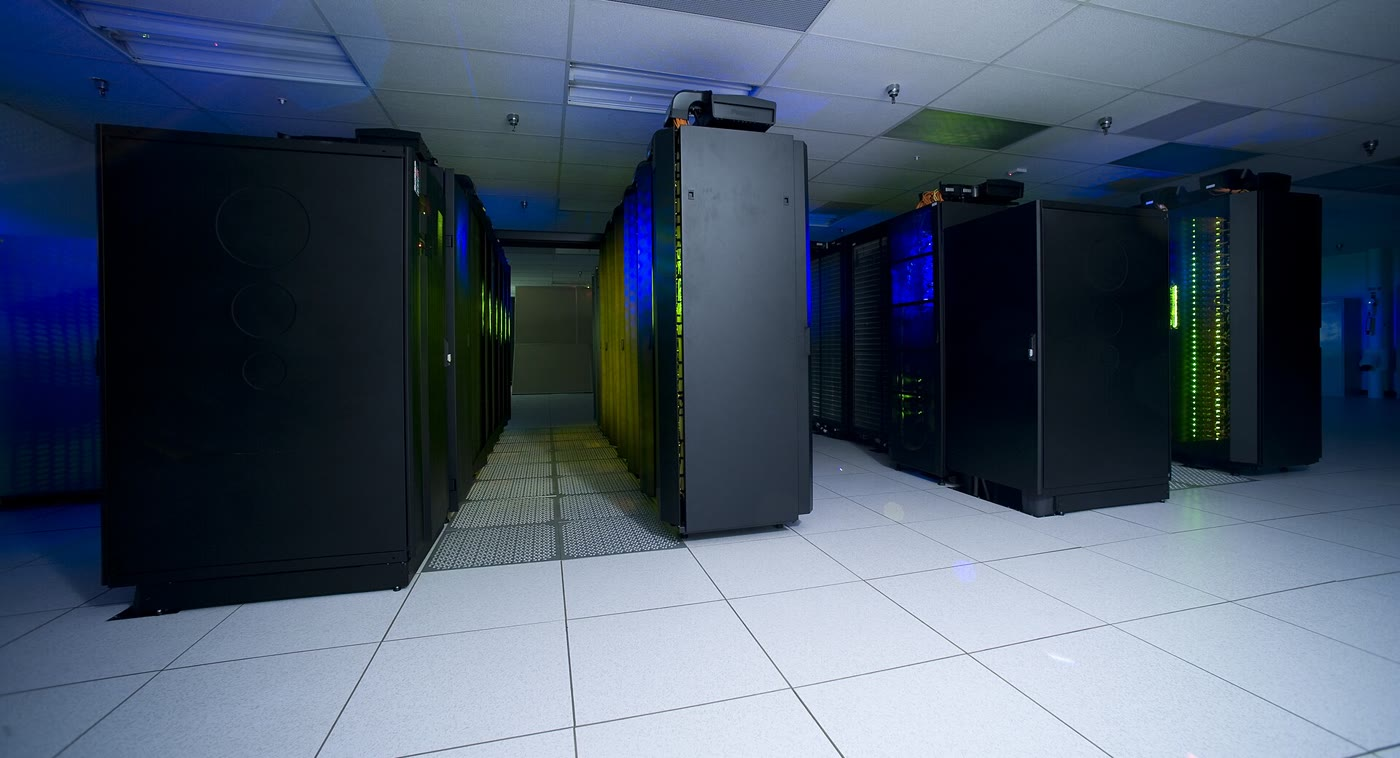
\includegraphics[width=0.7\linewidth]{images/book5/b3-nccs-supercomputer.jpg}

\par\smallskip{\small Rak-rak superkomputer di NASA Center for
Climate Simulation, Goddard Space Flight Center, pada 2010 (NASA, domain
publik). Persamaan model global diselesaikan secara numerik pada
komputer berkinerja tinggi semacam itu.}\label{fig:b3:climate-models:supercomputer}
\end{omfigure}
% ledger: photo:b3-nccs, ar6ch1:esm

\section{Mengevaluasi model}\label{sec:b3:climate-models:evaluation}

Model diuji terhadap iklim hasil pengamatan; masalahnya, model itu juga telah
disesuaikan dengannya. Setiap \omterm{def:b3:climate-models:gcm}{parameterisasi} memiliki parameter yang
rentang yang dapat diterima ditetapkan oleh fisika dan pengamatan, dan ketika komponen-komponen
dirakit, para pemodel menyempurnakannya hingga iklim hasil simulasi memenuhi
serangkaian target penyetelan: iklim rata-rata --- misalnya suhu rata-rata
yang dekat dengan nilai pengamatan di bawah sinar Matahari saat ini --- ciri regional, atau
tren pada periode historis. Barulah model dilepas untuk
perbandingan antarmodel.
% ledger: ar6ch1:models, ar6ch1:parameterization, ar6ch1:large-ensembles

\begin{definition}[Proyek perbandingan antarmodel]\label{def:b3:climate-models:cmip}
Yang disebut \emph{proyek perbandingan antarmodel}\index{proyek perbandingan antarmodel}
adalah serangkaian eksperimen terkoordinasi --- dengan forsing yang sama,
protokol yang sama, dan keluaran yang sama --- yang dijalankan banyak kelompok pemodelan
dengan model mereka sendiri agar hasilnya dapat dibandingkan. Coupled Model
Intercomparison Project (CMIP) berlangsung dalam fase-fase berurutan; fase keenamnya,
CMIP6, menjadi salah satu bukti utama asesmen keenam.
\end{definition}

\begin{dated}{2021}
Dari 29 kelompok pemodelan CMIP6 yang melaporkan cara mereka menyetel, 23 tidak
menyetel model mereka terhadap pemanasan yang teramati pada periode historis, dan
25 tidak menyetel ECS-nya: sensitivitas sebagian besar model merupakan sifat emergen
bukan masukan. Secara rata-rata, model CMIP6 memiliki ECS dan TCR yang lebih tinggi
daripada fase sebelumnya, dan sebaran yang lebih lebar daripada rentang
yang dinilai dalam laporan; pada beberapa model, hal ini ditelusuri ke umpan balik
awan di lintang menengah dan tinggi. Beberapa model paling sensitif
kurang mampu mereproduksi pemanasan terkini yang teramati dan iklim masa lalu
dengan baik. Oleh karena itu, asesmen tidak mengambil rentang ECS dan TCR-nya dari
model secara langsung, melainkan dari pemahaman tentang proses umpan balik,
catatan instrumental, iklim masa lalu, dan \omterm{def:b3:climate-models:evaluation}{kendala emergen}; asesmen memperlakukan model paling sensitif sebagai panduan
bagi hasil dengan kemungkinan rendah tetapi dampak tinggi (\emph{keyakinan tinggi}).
\end{dated}
% ledger: ar6ch1:models, ar6ch7:cmip6-sensitivity

\begin{definition}[Ansambel besar; kendala emergen]\label{def:b3:climate-models:evaluation}
Yang disebut \emph{ansambel besar}\index{ansambel besar} adalah sekumpulan banyak simulasi
dari satu model, dengan forsing yang sama selama periode yang sama, yang hanya berbeda
dalam keadaan awalnya. Yang disebut \emph{kendala
emergen}\index{kendala emergen} adalah hubungan yang ditemukan lintas
ansambel berbagai model, antara besaran yang teramati dari
iklim masa kini dan besaran iklim masa depan, seperti ECS; nilai
yang teramati dari besaran pertama lalu mempersempit rentang besaran kedua.
\end{definition}

Iklim bersifat kacau, sehingga perbedaan kecil pada keadaan awal membuat
anggota \omterm{def:b3:climate-models:evaluation}{ansambel besar} menempuh lintasan berbeda: sebaran anggota
mengukur variabilitas internal, dan rata-ratanya menunjukkan respons
akibat forsing. \omterm{def:b3:climate-models:evaluation}{Ansambel besar} dari beberapa model mendukung asesmen. Sebuah
\omterm{def:b3:climate-models:evaluation}{kendala emergen} memerlukan alasan fisis. Dengan beberapa lusin model,
ribuan besaran teramati dapat diuji, dan sebagian akan berkorelasi dengan
ECS secara kebetulan; asesmen hanya menyimpan yang berdasar fisis, banyak di antaranya
menyangkut awan di daerah tropis, dan memperingatkan bahwa bias yang dimiliki bersama oleh semua
model dalam ansambel itu menggagalkan metode ini.
% ledger: ar6ch1:large-ensembles, ar6ch7:emergent

\begin{inthelab}[Sebuah pusat pemodelan]
\begin{minipage}[t]{0.55\linewidth}\vspace{0pt}
Di pusat pemodelan iklim, model adalah program yang ditulis dan
dipelihara oleh sebuah tim: atmosfer, samudra, es laut, dan daratan merupakan komponen terpisah
komponen yang saling bertukar fluks di antarmukanya melalui penggandeng. Sebelum
model dijalankan, forsing eksperimen dimasukkan --- konsentrasi
gas rumah kaca, aerosol, dan tata guna lahan sesuai protokol. Bumi dibagi
menjadi bagian-bagian yang dihitung prosesor superkomputer secara paralel,
dan iklim model selama satu abad dihasilkan sebagai arsip besar
medan. Para ilmuwan menampilkannya di layar, membandingkannya dengan
reanalisis dan catatan satelit, lalu mengirim keluaran standar ke
arsip \omterm{def:b3:climate-models:cmip}{proyek perbandingan antarmodel}, tempat kelompok lain membandingkannya dengan milik mereka.
\end{minipage}\hfill
\begin{minipage}[t]{0.42\linewidth}\vspace{0pt}
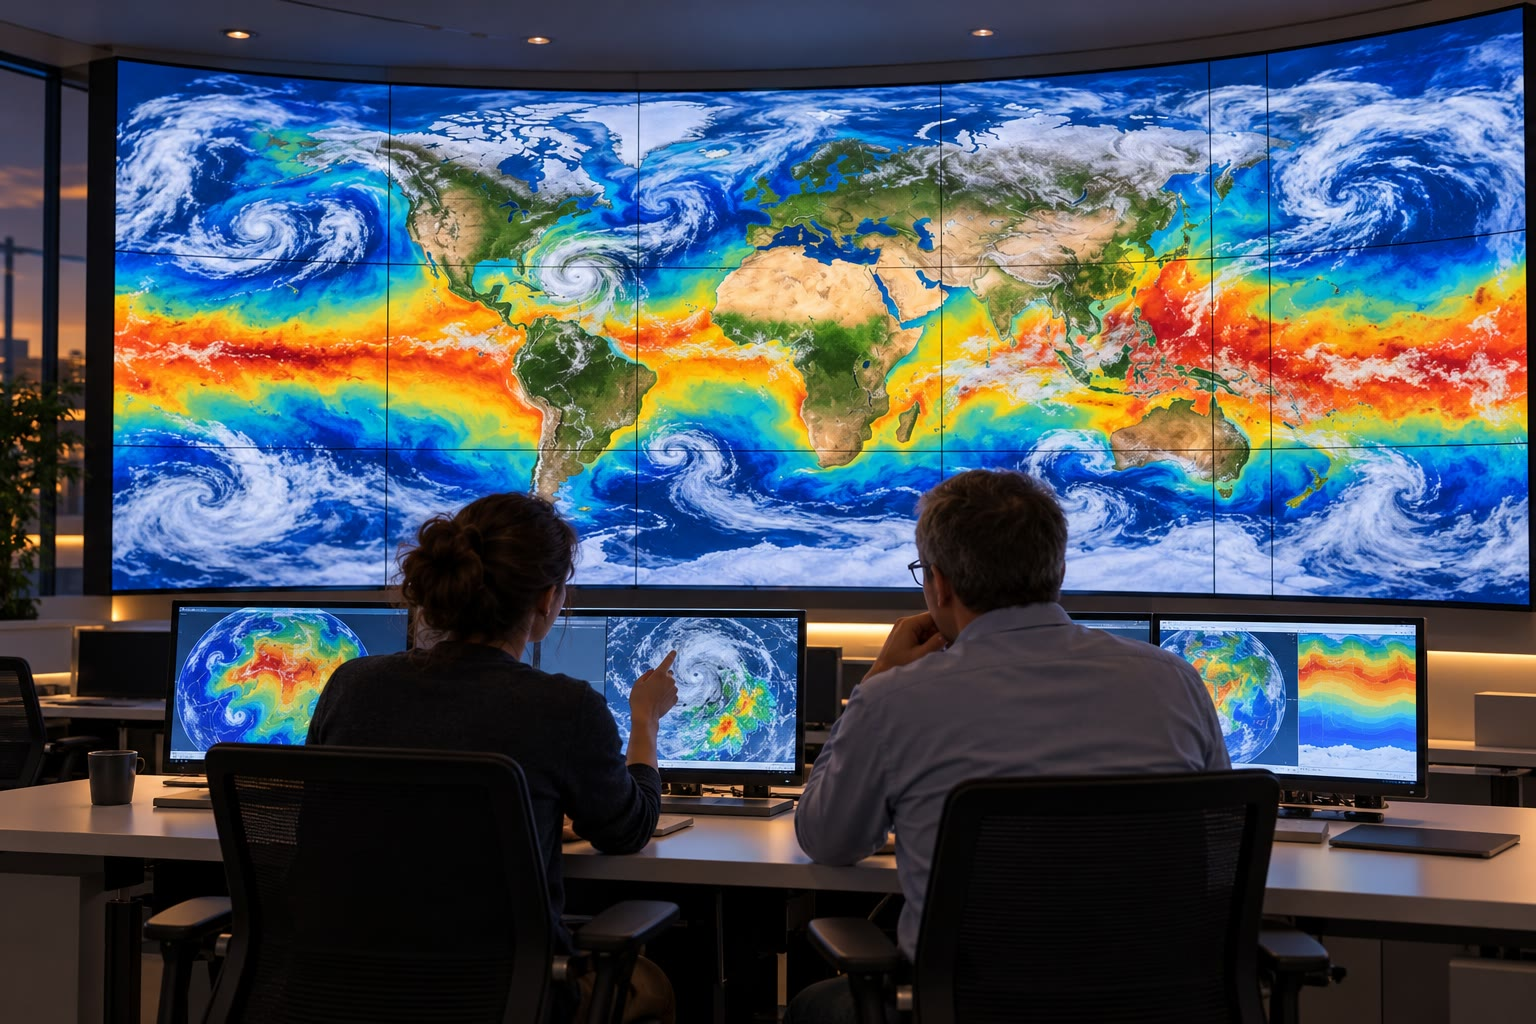
\includegraphics[width=\linewidth]{images/book5/ai/b3-model-centre.jpg}

{\scriptsize Dua ilmuwan di depan dinding layar yang menampilkan
medan global hasil simulasi model (ilustrasi buatan AI).}
\end{minipage}
\end{inthelab}
% ledger: ar6ch1:esm, ar6ch1:models

\section{Latihan}

\begin{exercise}[$\star$]\label{exo:b3:climate-models:1}
Hukum OLR Budyko adalah $I = a + bT - (a_1 + b_1T)n$, dengan $a = 14.0$, $b =
0.14$, $a_1 = 3.0$, $b_1 = 0.10$, dalam \unit{kcal.cm^{-2}} per bulan dan $T$
dalam \unit{\celsius}. Untuk tutupan awan $n = 0.5$, hitung $A$ dan $B$, dan
ubah keduanya ke \unit{W/m^2} dan \unit{W.m^{-2}.\celsius^{-1}}, dengan satu
bulan adalah seperduabelas dari tahun 365.25 hari. Berapa OLR yang diberikan hukum ini pada
\qty{15}{\celsius}?
\end{exercise}
% ledger: budyko69:olr

\begin{exercise}[$\star$]\label{exo:b3:climate-models:2}
Dengan $Q = \qty{340}{W/m^2}$, $A = \qty{211.9}{W/m^2}$ dan $B =
\qty{1.816}{W.m^{-2}.\celsius^{-1}}$, hitung suhu kesetimbangan
untuk albedo 0.30 dan 0.31. Seberapa besar planet ini mendingin bila
albedo naik 0.01?
\end{exercise}

\begin{exercise}[$\star$]\label{exo:b3:climate-models:3}
Hitung kapasitas panas per meter persegi lapisan campuran air laut
kedalaman \qty{60}{m}, $\rho = \qty{1025}{kg/m^3}$ dan $c_p = \qty{3992}{J.kg^{-1}.K^{-1}}$,
dalam \unit{J.m^{-2}.K^{-1}} dan dalam \unit{W.yr.m^{-2}.K^{-1}}. Hitung
waktu respons dari \cref{thm:b3:climate-models:response} untuk $\lambda = -B =
\qty{-1.816}{W.m^{-2}.\celsius^{-1}}$ dan untuk $\lambda =
\qty{-1.33}{W.m^{-2}.\celsius^{-1}}$.
\end{exercise}
% ledger: teos10:cp0

\begin{exercise}[$\star$]\label{exo:b3:climate-models:4}
Untuk model dua lapisan dengan $\lambda = \qty{-1.33}{W.m^{-2}.\celsius^{-1}}$,
$\gamma = \qty{0.62}{W.m^{-2}.\celsius^{-1}}$ dan $F_{2\times} =
\qty{3.93}{W/m^2}$, hitung ECS, TCR pendekatan $F_{2\times}/
(\gamma - \lambda)$, dan rasionya.
\end{exercise}
% ledger: ar6sm7:two-layer, ipcc:erf-2xco2

\begin{exercise}[$\star\star$]\label{exo:b3:climate-models:5}
Dalam model nol-dimensi pada teks ini, ambil konstanta surya sebesar
\qty{1340}{W/m^2}. Tentukan ketiga kesetimbangan serta kemiringan $N'(T)$
fluks neto di tiap kesetimbangan; mana yang stabil?
\end{exercise}

\begin{exercise}[$\star\star$]\label{exo:b3:climate-models:6}
Geser tanjakan albedo pada teks ini: $\alpha = 0.62$ di bawah \qty{-20}{\celsius},
$0.30$ di atas \qty{0}{\celsius}, dan berubah linear di antaranya. Pertahankan $A$ dan $B$. Pada konstanta surya berapa
cabang hangat berakhir, dan sebesar berapa persen itu di bawah
\qty{1360}{W/m^2}? Pada konstanta surya berapa bola salju mencair?
Apa yang menentukan besarnya ambang?
\end{exercise}

\begin{exercise}[$\star\star$]\label{exo:b3:climate-models:7}
Sebuah planet model dengan parameter pada teks ini berada dalam keadaan bola salju.
(a)~Berapa suhunya pada konstanta surya hari ini? (b)~Dengan Matahari dibiarkan
seperti adanya, gaya radiatif $F$ apa yang akan menaikkan suhu bola salju hingga
\qty{-10}{\celsius}? Berapa kali lipat gaya penggandaan karbon
dioksida, \qty{3.93}{W/m^2}, itu? (c)~Setelah es hilang, di mana planet
menetap jika gaya radiatif kemudian dihilangkan?
\end{exercise}
% ledger: ipcc:erf-2xco2, hoffman17:hysteresis

\begin{exercise}[$\star\star$]\label{exo:b3:climate-models:8}
Model X, sebuah model dua lapisan rekaan, memiliki $C = 7.0$ dan $C_d =
\qty{90}{W.yr.m^{-2}.\celsius^{-1}}$, $\gamma = 0.70$ dan $\lambda =
\qty{-1.10}{W.m^{-2}.\celsius^{-1}}$. Hitung kedua skala waktunya secara tepat
dan dengan pendekatan menurut \cref{thm:b3:climate-models:two-layer}, pecahan
$a_f$, ECS-nya, dan TCR pendekatannya.
\end{exercise}

\begin{exercise}[$\star\star$]\label{exo:b3:climate-models:9}
Dalam model Budyko pada teks ini, $\bar T = \qty{12.81}{\celsius}$, $\beta =
\qty{3.74}{W.m^{-2}.\celsius^{-1}}$, garis es pada \ang{72}, $s = 1.221$
di khatulistiwa dan $0.506$ di kutub, $\alpha = 0.30$ dan $0.62$.
Hitung suhu di khatulistiwa dan di kutub, serta panas
$\beta(T - \bar T)$ yang dikeluarkan transpor dari, atau dibawa ke, tiap
meter persegi di sana.
\end{exercise}

\begin{exercise}[$\star\star\star$]\label{exo:b3:climate-models:10}
Sebuah planet tanpa es ($\alpha = 0.30$ di mana-mana) memiliki transpor
difusif $D = -\mathcal D\,\partial_x[(1 - x^2)\partial_xT]$ dan
insolasi $s(x) = 1 + s_2P_2(x)$, $P_2 = (3x^2 - 1)/2$. (a)~Tunjukkan bahwa
$\partial_x[(1 - x^2)\partial_xP_2] = -6P_2$. (b)~Tunjukkan bahwa $T = T_0 +
T_2P_2(x)$ adalah solusi keadaan tunak, dengan $T_0 = (Q(1 - \alpha) - A)/B$ dan
$T_2 = Qs_2(1 - \alpha)/(B + 6\mathcal D)$. (c)~Insolasi
hasil reanalisis memberikan $s_2 = \num{-0.476}$. Tanpa transpor, berapa selisih suhu
antara khatulistiwa dan kutub? (d)~Berapa $\mathcal D$ yang memberikan
selisih yang teramati, \qty{55.3}{\celsius}?
\end{exercise}
% ledger: data:b3-ncep, data:b5-ncep-air

\begin{exercise}[$\star\star\star$]\label{exo:b3:climate-models:11}
(a)~Tulis persamaan kuadrat menurut \cref{thm:b3:climate-models:two-layer} sebagai $r^2 -
\Sigma r + \Pi = 0$ dan tunjukkan bahwa, jika $4\Pi \ll \Sigma^2$, akar-akarnya
dekat dengan $\Sigma$ dan $\Pi/\Sigma$. (b)~Untuk gaya radiatif $F = kt$ yang naik
secara linear, tunjukkan bahwa begitu $t \gg \tau_f$, dan selama $T_d$ tetap kecil,
$T \approx kt/(\gamma - \lambda)$; turunkan TCR pendekatannya. (c)~Periksa
angka-angka pada teks ini: $\Sigma$, $\Pi$, kedua skala waktu, dan
rasio $4\Pi/\Sigma^2$.
\end{exercise}
% ledger: ar6sm7:two-layer

\begin{exercise}[$\star\star\star$]\label{exo:b3:climate-models:12}
Sebuah ansambel rekaan berisi delapan model memberikan besaran teramati $X$
pada iklim masa kini dan ECS-nya:
\begin{center}
\begin{tabular}{l*{8}{c}}
\hline
$X$ & 0.2 & 0.5 & 0.6 & 0.8 & 1.0 & 1.1 & 1.3 & 1.5\\
ECS (\unit{\celsius}) & 2.3 & 2.7 & 3.1 & 3.2 & 3.8 & 3.9 & 4.4 & 4.6\\
\hline
\end{tabular}
\end{center}
(a)~Hitung rata-rata dan simpangan baku ECS
ansambel itu. (b)~Cocokkan ECS $= a + bX$ dengan kuadrat terkecil; hitung korelasi
dan simpangan baku residunya. (c)~$X$ teramati adalah $0.7
\pm 0.1$. Berapa ECS yang diberikan kendala ini, dan dengan sebaran berapa?
(d)~Apa yang membuatmu tidak percaya pada kendala ini?
\end{exercise}
% ledger: ar6ch7:emergent

\section{Soal: Seberapa dekat dengan bola salju?}

\begin{problem}[{Soal akhir pekan --- kesetimbangan, kestabilan dan
ambang glasiasi planet model}]
\label{pb:b3:climate-models:1}
Sebuah planet model memiliki konstanta surya hari ini $S_0 = \qty{1360}{W/m^2}$ dan
hukum OLR $A + BT$ dengan $A = \qty{211.9}{W/m^2}$ dan $B =
\qty{1.816}{W.m^{-2}.\celsius^{-1}}$. Albedonya 0.62 di bawah
\qty{-10}{\celsius}, 0.30 di atas \qty{+10}{\celsius}, linier di antaranya, dan
kapasitas panas permukaannya $C = \qty{8.1}{W.yr.m^{-2}.\celsius^{-1}}$. Gunakan
$\sigma = \qty{5.670e-8}{W.m^{-2}.K^{-4}}$.

\medskip\noindent\textbf{Bagian I --- Planet dalam kesetimbangan.}
\begin{enumerate}
\item Hitung rata-rata sinar matahari $Q_0$ per meter persegi planet, dan
  jelaskan faktornya.
\item Hitung sinar matahari yang diserap dengan albedo 0.30, dan OLR pada
  \qty{15}{\celsius}.
\item Hitung kesetimbangan hangat.
\item Hitung kesetimbangan bola salju, dan periksa bahwa ia berada pada
  cabang es.
\item Hitung kesetimbangan ketiga, pada tanjakan albedo.
\item Hitung suhu emisi yang mengembalikan sinar matahari yang diserap
  ke angkasa sebagai benda hitam, dan bandingkan dengan kesetimbangan hangat.
\end{enumerate}

\medskip\noindent\textbf{Bagian II --- Kestabilan dan waktu.}
\begin{enumerate}[resume]
\item Hitung kemiringan $N'(T)$ dari fluks neto pada setiap kesetimbangan, dan
  nyatakan mana yang stabil.
\item Simpangan kecil dari kesetimbangan tengah tumbuh sebagai $\mathrm
  e^{t/\tau}$. Hitung $\tau$.
\item Hitung waktu respons kesetimbangan hangat.
\item Gaya radiatif sebesar \qty{3.93}{W/m^2}, setara dengan penggandaan
  karbon dioksida, mulai diberikan. Hitung pemanasan pada kesetimbangan, dan bandingkan
  dengan ECS yang ditaksir untuk iklim nyata.
\item Berapa lama model memerlukan waktu untuk mencapai \qty{95}{\percent} dari
  pemanasan? Mengapa iklim nyata membutuhkan waktu lebih lama?
\end{enumerate}

\medskip\noindent\textbf{Bagian III --- Bifurkasi pelana-simpul.}
\begin{enumerate}[resume]
\item Ketika Matahari meredup, pada suhu berapa kesetimbangan hangat bertemu
  dengan kesetimbangan tengah? Hitung $Q$ di sana.
\item Hitung konstanta surya pada bifurkasi, dan penurunannya dari
  hari ini dalam persen.
\item Tepat di bawahnya, ke mana iklim bergerak? Hitung suhunya.
\item Hitung konstanta surya saat bola salju mencair, dan kenaikannya
  dari hari ini dalam persen.
\item Sketsakan lengkung yang dilalui suhu ketika $S_0$ diturunkan
  di bawah bifurkasi dan dikembalikan ke \qty{1360}{W/m^2}.
\end{enumerate}

\medskip\noindent\textbf{Bagian IV --- Garis es.} Berikan model lintang Budyko
untuk planet ini, dengan $\beta = \qty{3.739}{W.m^{-2}.\celsius^{-1}}$,
albedo es 0.62 di sisi kutub garis es, 0.30 di sisi khatulistiwa, 0.50 pada
tepinya, dan insolasi dari reanalisis:
\begin{center}
\begin{tabular}{lccccccc}
\hline
lintang & \ang{0} & \ang{30} & \ang{40} & \ang{47.5} & \ang{55} & \ang{60} & \ang{72}\\
$s(x_s)$ & 1.2211 & 1.0730 & 0.9647 & 0.8688 & 0.7650 & 0.6947 & 0.5643\\
$F(x_s)$ & 0 & 0.5865 & 0.7324 & 0.8192 & 0.8863 & 0.9205 & 0.9738\\
\hline
\end{tabular}
\end{center}
\begin{enumerate}[resume]
\item Dengan garis es pada \ang{72}, hitung albedo rata-rata $\bar\alpha$
  dan suhu rata-rata $\bar T$.
\item Hitung suhu kritis $T_c$ yang menempatkan tepi pada
  \ang{72} hari ini, dan bandingkan dengan reanalisis, \qty{-15.8}{\celsius}.
\item Hitung pembilang dari $Q(x_s)$ pada \cref{prop:b3:climate-models:iceline}
  dan rasio $\beta/B$.
\item Hitung $Q(x_s)/Q_0$ untuk garis es pada \ang{30}, \ang{40},
  \ang{47.5}, \ang{55}, dan \ang{60}.
\item Di mana nilai minimum dari nilai-nilai ini berada? Garis es mana yang stabil?
\item Dengan Matahari hari ini, garis es lain apa yang diizinkan model, dan apakah
  itu stabil? Apakah bola salju mungkin hari ini? (Gunakan kolom \ang{0}.)
\item Bandingkan ambang model lintang dengan ambang Bagian~III
  dan \qty{1.6}{\percent} milik Budyko, dan lintang es pada
  ambang dengan \ang{50} miliknya.
\item Berikan, hingga dua angka penting, penurunan konstanta surya, dalam
  persen, yang menyebabkan glasiasi pada planet model.
\end{enumerate}
\end{problem}
% ledger: nasa:solar-mean, data:b5-ncep-air, data:b3-ncep, budyko69:transport, budyko69:albedo, budyko69:threshold, ipcc:ecs, const:sigma
